\documentclass[12pt]{article}

\title{A visual method for generating the separating isosurface of two classes of objects in two-dimensional space}
\author{
Shawn Halayka\footnote{Independent -- sjhalayka@gmail.com}
}


\date{\today\;\currenttime}

\usepackage{datetime}
\usepackage{listings}
\usepackage{cite}
\usepackage{xcolor}
\usepackage{graphicx}
\usepackage{setspace}
\usepackage{amsmath}
\usepackage{url}
\usepackage{amsfonts}
\usepackage{caption}
\usepackage{subcaption}

\usepackage[margin=1in]{geometry}

%\doublespace

\begin{document}




\maketitle

\begin{abstract}
With regard to the separating isosurface of two classes of objects in two-dimensional space, the transition from nonlinear to linear is documented. OpenCV and Marching Squares were used to calculate the data used for illustrations in this paper.
\end{abstract}




\section{Introduction}


Marching Squares works as a radial isosurface generator, as well as a linear isosurface generator.
Balance between high variance (curvilinear) and high bias (rectilinear).
OpenCV was used to downsize the image.
OpenCV can also be used to transform an image via blur, sharpen, or whatnot -- this visual method practically begs for such experimentation.





\begin{thebibliography}{9}

\bibitem{mc} James, et al. An Introduction to Statistical Learning with Applications in R. ISBN: 978-1-0716-1417-4

\end{thebibliography}










\begin{figure} 
\centering
  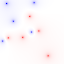
\includegraphics[width = 3 in]{64_res_image.png}
  \caption{Bitmap image used as input to the Marching Squares algorithm. 
Image size is 64x64.
Colour falls of with distance.
}
\end{figure}

\begin{figure} 
\centering
  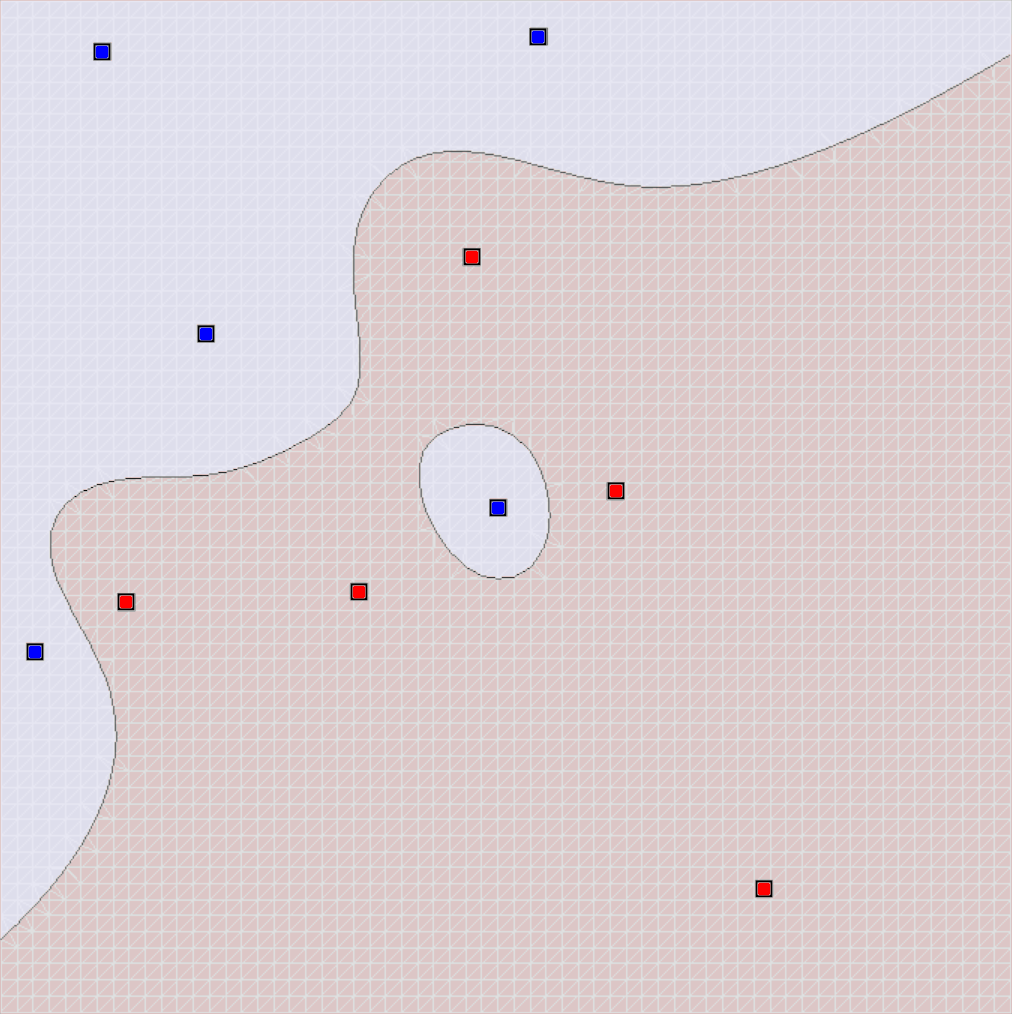
\includegraphics[width = 3 in]{64_res.png}
  \caption{Nonlinear, radial separation. Grid resolution is 64x64.
}
\end{figure}


\begin{figure} 
\centering
  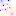
\includegraphics[width = 3 in]{16_res_image.png}
  \caption{Bitmap image used as input to the Marching Squares algorithm.
Image size is 16x16.
}
\end{figure}


\begin{figure} 
\centering
  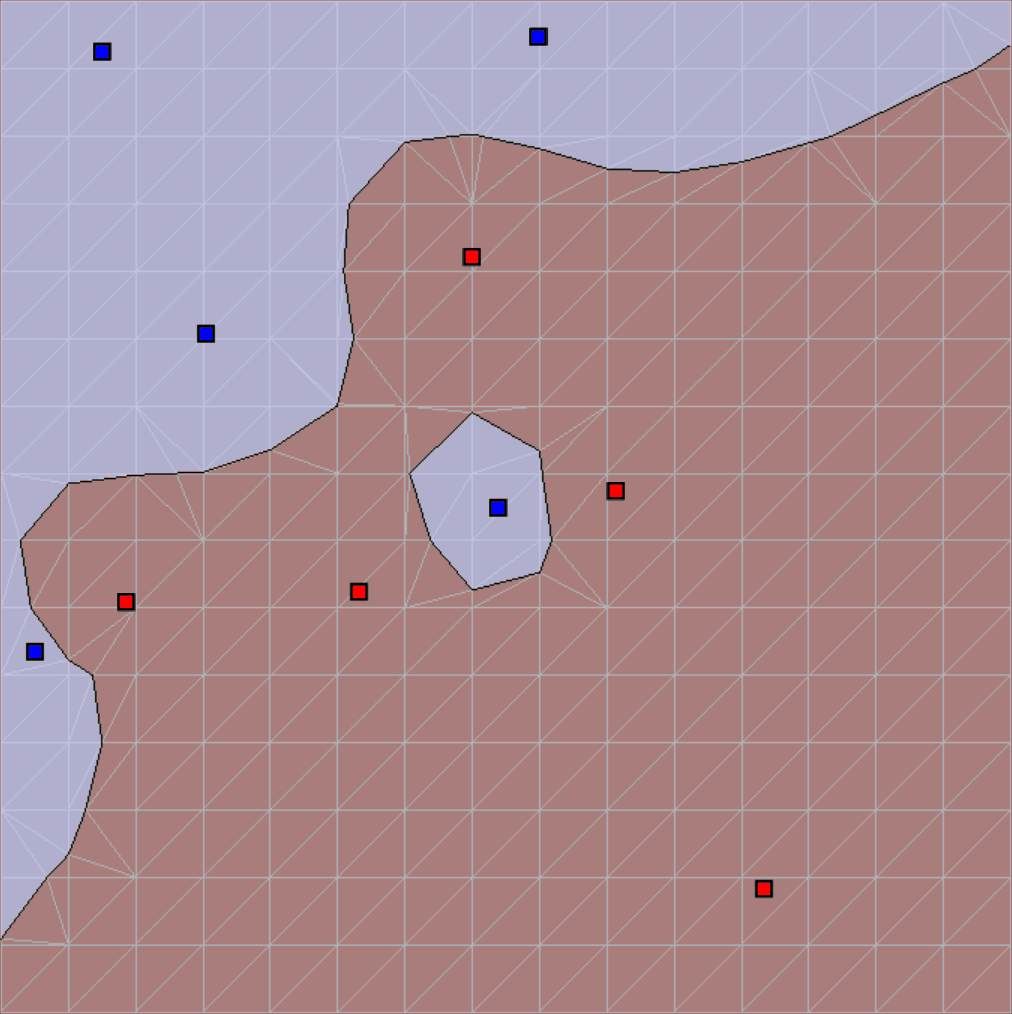
\includegraphics[width = 3 in]{16_res.png}
  \caption{Nonlinear, radial separation. Grid resolution is 16x16.
}
\end{figure}

\begin{figure} 
\centering
  
\includegraphics[width = 3 in]{2_res_image.png}
  \caption{Bitmap image used as input to the Marching Squares algorithm.
Image size is 2x2.
}
\end{figure}


\begin{figure} 
\centering
  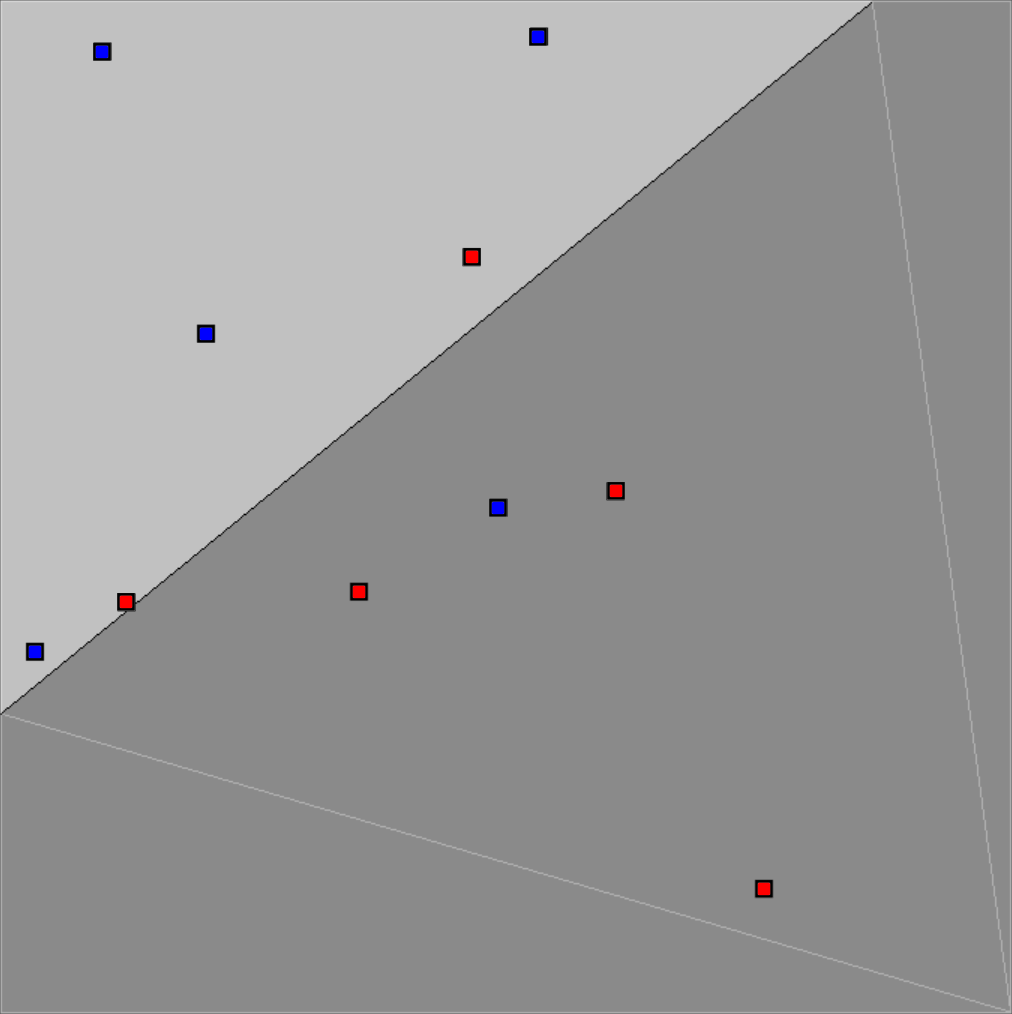
\includegraphics[width = 3 in]{2_res.png}
  \caption{Linear separation. Grid resolution is 2x2.
}
\end{figure}












\end{document}









